\documentclass[11pt]{article}

\usepackage[margin=1in]{geometry}
\usepackage[utf8]{inputenc}
\usepackage[T1]{fontenc}
\usepackage{charter}
\usepackage{amsmath,amssymb}
\usepackage{booktabs}
\usepackage[numbers]{natbib}
\usepackage{float}
\usepackage{xurl}
\usepackage{hyperref}
\usepackage{enumitem}
\usepackage{caption}
\usepackage{titlesec}
\usepackage{xcolor}
\usepackage{tikz}
\usetikzlibrary{positioning,arrows.meta,fit}

\hypersetup{colorlinks=true,linkcolor=black,citecolor=black,urlcolor=blue!50!black}
\titleformat{\section}{\normalfont\large\bfseries}{\thesection}{0.6em}{}
\titleformat{\subsection}{\normalfont\bfseries}{\thesubsection}{0.6em}{}
\captionsetup{font=small,skip=4pt}
\setlength{\textfloatsep}{10pt plus 2pt minus 2pt}

\title{\textbf{Fostering Epistemic Diversity in the AI Era}\\
\large A Map of Ideas, a Measure, and a First Experiment}

\author{
Sofia G. Gallego$^{1}$ \\[4pt]
\normalsize $^1$CosmoVentures, Paris, France, with Apart Research
}
\date{Apart Research AI $\times$ Epistemics Research Sprint, November 2026}

\begin{document}
\maketitle

\begin{abstract}
As more thinking passes through AI, the range of ideas people meet can narrow without anyone noticing. Tools built on what is already written tend to converge on what is already known, and help from AI can make each person's ideas better while making a group's ideas more alike. We propose a program for the opposite direction: ways of working with AI that widen the ideas people reach. It has three parts that check one another. A measure: Epistemic Bridges, a game in which people and models link the same words, places any model or tool on a map drawn by real people, with recall and precision and without a model as judge. A tool: the Map of Ideas (mapideas.org), a public map where concepts and debates are seen from many perspectives and the space between them is visible. Changes to models: in Bridges, giving a model the perspective of an ordinary person was the only change that widened its ideas on every model. During the sprint we built the measure and designed a first experiment that uses it to test the tool: do people who explore the map, or work with an AI, reach more of the space of ideas than people alone, or do they converge on what they were shown?
\end{abstract}

\section{Introduction}

Epistemic diversity is how a group notices its own mistakes, finds new ideas and keeps a debate alive. Groups of people who think differently can find solutions that groups of the individually best problem solvers miss \citep{hong2004}. Much of that diversity lives in the space between ideas: the same concept reads differently to a physicist, a poet and a cook, and new connections often appear where those readings meet.

AI is becoming a shared layer of that thinking. Chat training reduces the variety of what a model writes \citep{kirk2024}, models are more alike in their creative output than people are \citep{wenger2026,jiang2025}, and help from AI can improve each person's ideas while making the ideas of a group more alike \citep{doshi2024,anderson2024}. If people rely on the same models for the same questions, rarer ideas can fade from use, a process described as knowledge collapse \citep{peterson2024,wright2025}. None of this is fixed. The same tools could also be built to open the space, by showing contrasting views, by bringing in perspectives a person would not reach alone, and by keeping track of what is lost.

This report sets out a program for fostering epistemic diversity with AI, and the first steps taken during the sprint. It rests on three parts (Figure~\ref{fig:program}):
\begin{enumerate}[itemsep=0.1em]
\item \textbf{A measure} of how much of the space of ideas a person, a model or a tool reaches, grounded in what real people do.
\item \textbf{Tools for people} that make the space between ideas visible, starting with the Map of Ideas.
\item \textbf{Changes to models} that widen what they reach, and loosen the one voice that chat models share.
\end{enumerate}
The measure is the part that keeps the others honest: any tool or model change can look diverse while narrowing what people actually reach, so each one is checked against the same human map.

\begin{figure}[H]
\centering
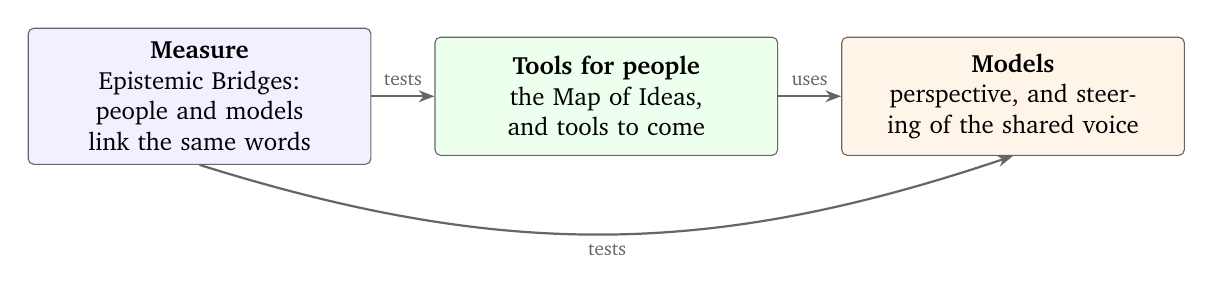
\begin{tikzpicture}[node distance=6mm and 8mm, every node/.style={font=\small},
  box/.style={draw=black!60, rounded corners=2pt, align=center, inner sep=5pt, text width=4.0cm, minimum height=1.5cm},
  arr/.style={-{Stealth[length=2mm]}, black!60, thick}]
\node[box, fill=blue!6] (m) {\textbf{Measure}\\ Epistemic Bridges: people and models link the same words};
\node[box, fill=green!7, right=of m] (t) {\textbf{Tools for people}\\ the Map of Ideas, and tools to come};
\node[box, fill=orange!9, right=of t] (a) {\textbf{Models}\\ perspective, and steering of the shared voice};
\draw[arr] (m) -- node[above, font=\scriptsize]{tests} (t);
\draw[arr] (m.south) to[bend right=18] node[below, font=\scriptsize]{tests} (a.south);
\draw[arr] (t) -- node[above, font=\scriptsize]{uses} (a);
\end{tikzpicture}
\caption{The program and how its parts relate. The measure, built on what real people do, tests both the tools for people and the changes to models; the tools can use the models that widen.}
\label{fig:program}
\end{figure}

\section{Related Work}

\textbf{Homogenization and knowledge collapse.} Evidence that AI narrows ideas comes from models \citep{kirk2024,wenger2026,jiang2025,zhang2025} and from people working with them \citep{doshi2024,anderson2024}. Knowledge collapse describes how reliance on AI can shrink the range of knowledge in use over time \citep{peterson2024}, and has been measured across models and languages \citep{wright2025}.

\textbf{Maps of opinions and ideas.} Polis maps the opinions of many people so that groups see where they agree and differ, and has been used in public deliberation \citep{polis2021}. The Map of Ideas shares the aim of making a space visible, and applies it to concepts and how they read from each other, across disciplines.

\textbf{Measuring diversity against people.} Most measures ask how much a set of answers varies. Epistemic Bridges asks how much of the ground that people cover a model reaches, adapting precision and recall from generative models \citep{kynkaanniemi2019}, and separates the shared voice of chat models from their ideas \citep{shaib2024}.

\section{The Map of Ideas}

The Map of Ideas (\href{https://mapideas.org}{mapideas.org}) is a public, wiki-style map where ideas grow and relate. It existed before the sprint; we describe it here because it is the first tool of the program. It started from Gödel and now holds more than 200 ideas and about 100 open questions across 17 topics, from mathematics and astronomy to religions, cultures and art. Several of its choices come from the goal of diversity:
\begin{itemize}[itemsep=0.1em]
\item \textbf{Readings in both directions.} A link can carry how one idea reads when you come from the other, so a connection is seen from both sides.
\item \textbf{Answers and open questions.} An answer is a full idea joined to the one it answers, with its own sources, so a debate shows its views side by side. Open questions sit between topics.
\item \textbf{Care for traditions.} Each tradition, people and culture has its own idea, described as its own followers would, and nothing is ranked.
\item \textbf{Re-centering.} Any idea can become the center, so the map has no single starting point.
\item \textbf{A guide that never writes.} An AI guide answers questions from the ideas on the map and does not add to it. What is on the map was written by people, with sources and a full history.
\end{itemize}

A map shown to everyone is itself a shared prior. It could widen what people reach, or it could become the new common answer. That is the question the measure lets us test.

\section{What Bridges Shows}

During the sprint, Epistemic Bridges \citep{gallego2026bridges} gave the program its measure and its first evidence. In the game, people link two words with no evident connection, in any form. The players' answers draw a map of where people go, and each model is placed on it by recall (how much of the map it reaches) and precision (how many of its answers land on it). With 27 players and 15 open models, measured as written, chat models seem to reach almost none of the map. Most of that gap is one shared voice. With the voice removed from every answer in the same way, the larger and newer chat models still reach less of the map than people (recall 47\% to 59\%, against 81\%), and no model comes near people on both counts. Reasoning personas mostly change the voice, and one narrows the ideas. Only one condition widened the ideas on every model: answering as an ordinary person drawn at random. A reasoning persona held by such a life widened them too.

Two lessons carry into the program. Diversity has to be measured with the voice and the ideas apart, or a tool can look diverse by changing how things are said. And perspective is what moved the models toward where people go.

\section{A First Experiment: Does a Tool Widen What People Reach?}

The new step designed during the sprint uses the Bridges measure on people instead of models. Players receive the same pairs as in Bridges and are assigned at random to one of four conditions (Figure~\ref{fig:design}):
\begin{enumerate}[itemsep=0.1em]
\item \textbf{Alone}, as in the game today.
\item \textbf{With the map}: before answering, the player explores the Map of Ideas for a short time, centered on ideas near the two words.
\item \textbf{With an AI}: the player sees one AI bridge before answering, from a chat model with no persona.
\item \textbf{With an AI given a perspective}: the same, from the same model answering as an ordinary person drawn at random.
\end{enumerate}

The reference map is drawn by a separate group of players who answer alone and are never compared with themselves. Each condition is then described as a group, as models are in Bridges: recall, how much of the reference map its answers reach; precision, how many of its answers land on it; and the voice, how much its sentence patterns repeat. The main question is whether recall at the group level goes up or down. A tool that helps each person but pulls everyone toward what they were shown will raise individual answers while lowering group recall, the pattern seen in earlier studies \citep{doshi2024}. The design can tell these apart.

\begin{figure}[H]
\centering
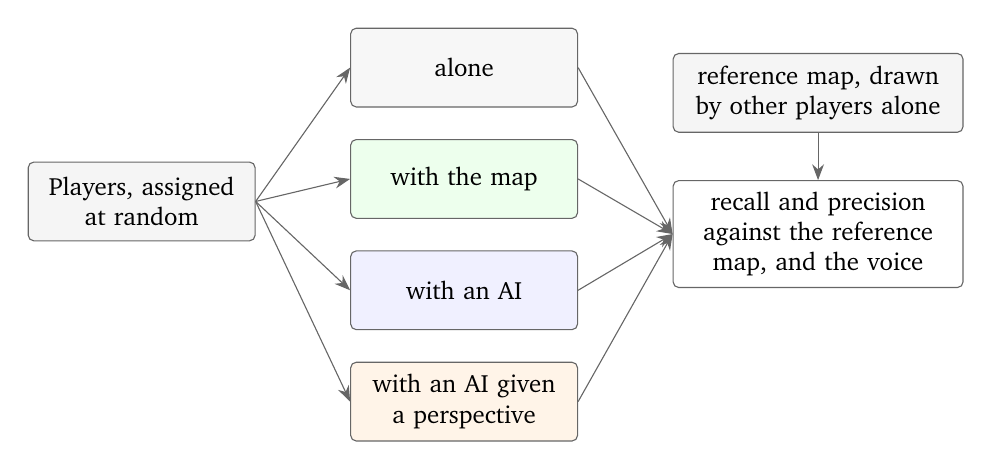
\begin{tikzpicture}[node distance=4mm and 8mm, every node/.style={font=\small},
  arm/.style={draw=black!60, rounded corners=2pt, align=center, inner sep=4pt, text width=2.6cm, minimum height=1.0cm},
  arr/.style={-{Stealth[length=2mm]}, black!60}]
\node[arm, fill=black!4] (p) {Players, assigned at random};
\node[arm, right=12mm of p, yshift=17mm, fill=black!3] (a1) {alone};
\node[arm, below=of a1, fill=green!7] (a2) {with the map};
\node[arm, below=of a2, fill=blue!6] (a3) {with an AI};
\node[arm, below=of a3, fill=orange!9] (a4) {with an AI given a perspective};
\node[arm, right=12mm of a2, yshift=-7mm, text width=3.4cm] (r) {recall and precision against the reference map, and the voice};
\node[arm, above=6mm of r, text width=3.4cm, fill=black!4] (ref) {reference map, drawn by other players alone};
\foreach \n in {a1,a2,a3,a4} {\draw[arr] (p.east) -- (\n.west); \draw[arr] (\n.east) -- (r.west);}
\draw[arr] (ref) -- (r);
\end{tikzpicture}
\caption{Design of the first experiment. Each condition is described as a group, against a reference map drawn by players who answer alone, so a tool that makes everyone answer alike shows up as lower recall even when each answer looks good.}
\label{fig:design}
\end{figure}

\textbf{Size.} Bridges reached its first results with 27 players. Tools are likely to make smaller differences than the gap between people and models, so a first estimate is around 60 players per condition and for the reference group, 300 in all, to be set by a power analysis on the Bridges data before the experiment starts. The game already runs in five languages, without accounts, cookies or IP addresses, and the conditions need only small changes to it.

\textbf{What would count as success.} A tool fosters epistemic diversity if, at the group level, it raises recall without lowering precision, and if it does so with the voice removed. A tool that raises precision while lowering recall is making people more alike, however good each answer looks.

\section{Conclusion and Future Work}

Fostering epistemic diversity needs to see the space of ideas, to have tools that open it, and to have models that do not narrow it. During the sprint the first of these became concrete: a measure grounded in real people, which already showed that chat models narrow the space and that perspective can widen it. The next steps follow from it: run the experiment above; let players see, after answering, where their own connection sits among everyone's on the Map of Ideas; add frontier models and more languages to the measure; steer the shared voice inside models, which we began for a separate hackathon; and test whether perspective also helps models catch the blind spots they share \citep{gallego2026fer}. The longer aim is a harmonic relation between people and AI, where each widens what the other can reach.

\textbf{Limitations.} The experiment is a design and has not been run. Bridges uses 27 players and simple word pairs; whether its measure carries to research, debate or policy is open. The Map of Ideas is a young project, written in English, and many of its descriptions still need checking by people from each field and tradition.

\section*{Data and Code Availability}
The Bridges measure, AI answers and analysis are at \url{https://github.com/nefinia/epistemic-bridges}, with this report in the \texttt{fostering/} folder. The game is at \url{https://mapideas.org/bridges} and the map at \url{https://mapideas.org}. The Map of Ideas and the Bridges game existed before the sprint started on 13 November; the measure, its results and the experiment design were made during it.

\section*{Author Contributions and Acknowledgements}
S.G.G.\ designed the program, the map, the game and the experiment, and wrote the report with Claude (see LLM Usage Statement). Thanks to everyone who played Bridges and left feedback.

\begin{thebibliography}{99}
\small
\bibitem{hong2004} L.\ Hong, S.\ E.\ Page. \emph{Groups of diverse problem solvers can outperform groups of high-ability problem solvers.} PNAS, 101(46), 2004.
\bibitem{kirk2024} R.\ Kirk, I.\ Mediratta, C.\ Nalmpantis, J.\ Luketina, E.\ Hambro, E.\ Grefenstette, R.\ Raileanu. \emph{Understanding the Effects of RLHF on LLM Generalisation and Diversity.} ICLR, 2024.
\bibitem{wenger2026} E.\ Wenger, Y.\ N.\ Kenett. \emph{Large language models are homogeneously creative.} PNAS Nexus, 5(3):pgag042, 2026.
\bibitem{jiang2025} L.\ Jiang et al. \emph{Artificial Hivemind: The Open-Ended Homogeneity of Language Models (and Beyond).} NeurIPS, 2025.
\bibitem{doshi2024} A.\ R.\ Doshi, O.\ P.\ Hauser. \emph{Generative AI enhances individual creativity but reduces the collective diversity of novel content.} Science Advances, 10(28), 2024.
\bibitem{anderson2024} B.\ R.\ Anderson, J.\ H.\ Shah, M.\ Kreminski. \emph{Homogenization Effects of Large Language Models on Human Creative Ideation.} Creativity \& Cognition, 2024.
\bibitem{peterson2024} A.\ J.\ Peterson. \emph{AI and the Problem of Knowledge Collapse.} arXiv:2404.03502, 2024.
\bibitem{wright2025} D.\ Wright, S.\ Masud, J.\ Moore, S.\ Yadav, M.\ Antoniak, P.\ Ebert Christensen, C.\ Y.\ Park, I.\ Augenstein. \emph{Epistemic Diversity and Knowledge Collapse in Large Language Models.} arXiv:2510.04226, 2025.
\bibitem{zhang2025} Y.\ Zhang, H.\ Diddee, S.\ Holm, H.\ Liu, X.\ Liu, V.\ Samuel, B.\ Wang, D.\ Ippolito. \emph{NoveltyBench: Evaluating Language Models for Humanlike Diversity.} arXiv:2504.05228, 2025.
\bibitem{polis2021} C.\ Small, M.\ Bjorkegren, T.\ Erkkilä, L.\ Shaw, C.\ Megill. \emph{Polis: Scaling Deliberation by Mapping High Dimensional Opinion Spaces.} Recerca, 26(2), 2021.
\bibitem{kynkaanniemi2019} T.\ Kynkäänniemi, T.\ Karras, S.\ Laine, J.\ Lehtinen, T.\ Aila. \emph{Improved Precision and Recall Metric for Assessing Generative Models.} NeurIPS, 2019.
\bibitem{shaib2024} C.\ Shaib, Y.\ Elazar, J.\ J.\ Li, B.\ C.\ Wallace. \emph{Detection and Measurement of Syntactic Templates in Generated Text.} EMNLP, 2024.
\bibitem{gallego2026bridges} S.\ G.\ Gallego. \emph{Epistemic Bridges: Do Language Models Reach the Connections People Make?} Apart Research AI $\times$ Epistemics Research Sprint, 2026. \url{https://github.com/nefinia/epistemic-bridges}
\bibitem{gallego2026fer} S.\ G.\ Gallego, A.\ Habana. \emph{False Epistemic Redundancy: Do AI Ensembles Share a Blind Spot?} Apart Research Digital Minds Research Sprint, 2026. \url{https://apartresearch.com/project/false-epistemic-redundancy-do-ai-ensembles-share-a-blind-spot-b50u}
\end{thebibliography}

\section*{LLM Usage Statement}
Claude helped build the Map of Ideas and the Bridges game before the sprint and, during it, helped write the Bridges analysis and drafted and revised this report with the author, including the experiment design and the diagrams. All numbers about Bridges come from its analysis scripts and paper.

\end{document}
